\documentclass[a4paper]{article}
\usepackage[letterpaper,top=2cm,bottom=2cm,left=3cm,right=3cm,marginparwidth=1.75cm]{geometry}
\usepackage[colorlinks=true, allcolors=blue]{hyperref}

\usepackage{wrapfig}
\usepackage{amsthm}
\usepackage{hyperref}
\usepackage{graphicx}
\usepackage{amsfonts}

\title{Homework 2: Krylov Methods}
\author{Patryk Drozd}
\begin{document}
\date{}
\maketitle

\section*{Overview}
	I managed to get the first 2 questions done, however due to not being able to debug probably 
	something really stupid in time for the deadline, I didnt get a correct working parallel version of
	gmres.
		
	The code structure contains serial python code for parts 2.1 and 2.2. The main functions are found
	inside the functions.py file and the code to produce results for parts 2.1 and 2.2 are found in 
	files names q1.py and q2.py respectively. For part 2.3 I have not fully functioning c code for 
	the gmres algorithm in serial\_gmres.c , along with a makefile which is builds some parts of the
	code.

\section*{2.1}
	
	For this first question results are obatined with the following command.
	
	\begin{verbatim}
	drozdtux@Copernicus $ python q1.py
	[ 0.1566404  -0.06878725  0.33805709 -0.14304807 -0.06380229  0.51011703
	 -0.2996666   0.11218223  0.12160961 -0.67418307]
	\end{verbatim}

	This shows $Q_9$ in array form.

\section*{2.2}
	
	For the serial implementation of GMRES in python I chose to follow Algorithm 6.9 from 
	\textit{Iterative Methods for Sparse Linear Systems by Yousef Saad}. I couldnt quite figure
	out how to write the last line of Algorithm 6.9 to get a resuidual at every step. In my
	implementation modified the shapes of h and v in order to calculate the residuals for which 
	the graph I obain looks correct.

	Figure 1 shows for $n = 8, 16, 32, 64, 128, 256$ the serial gmres function run
	for $m = n/2$ iterations. From the plot we can see that the convergce rate doesnt depend on n
	since all of the lines appear to have the same slope.
	\begin{figure}[h!]
	    \centering
    	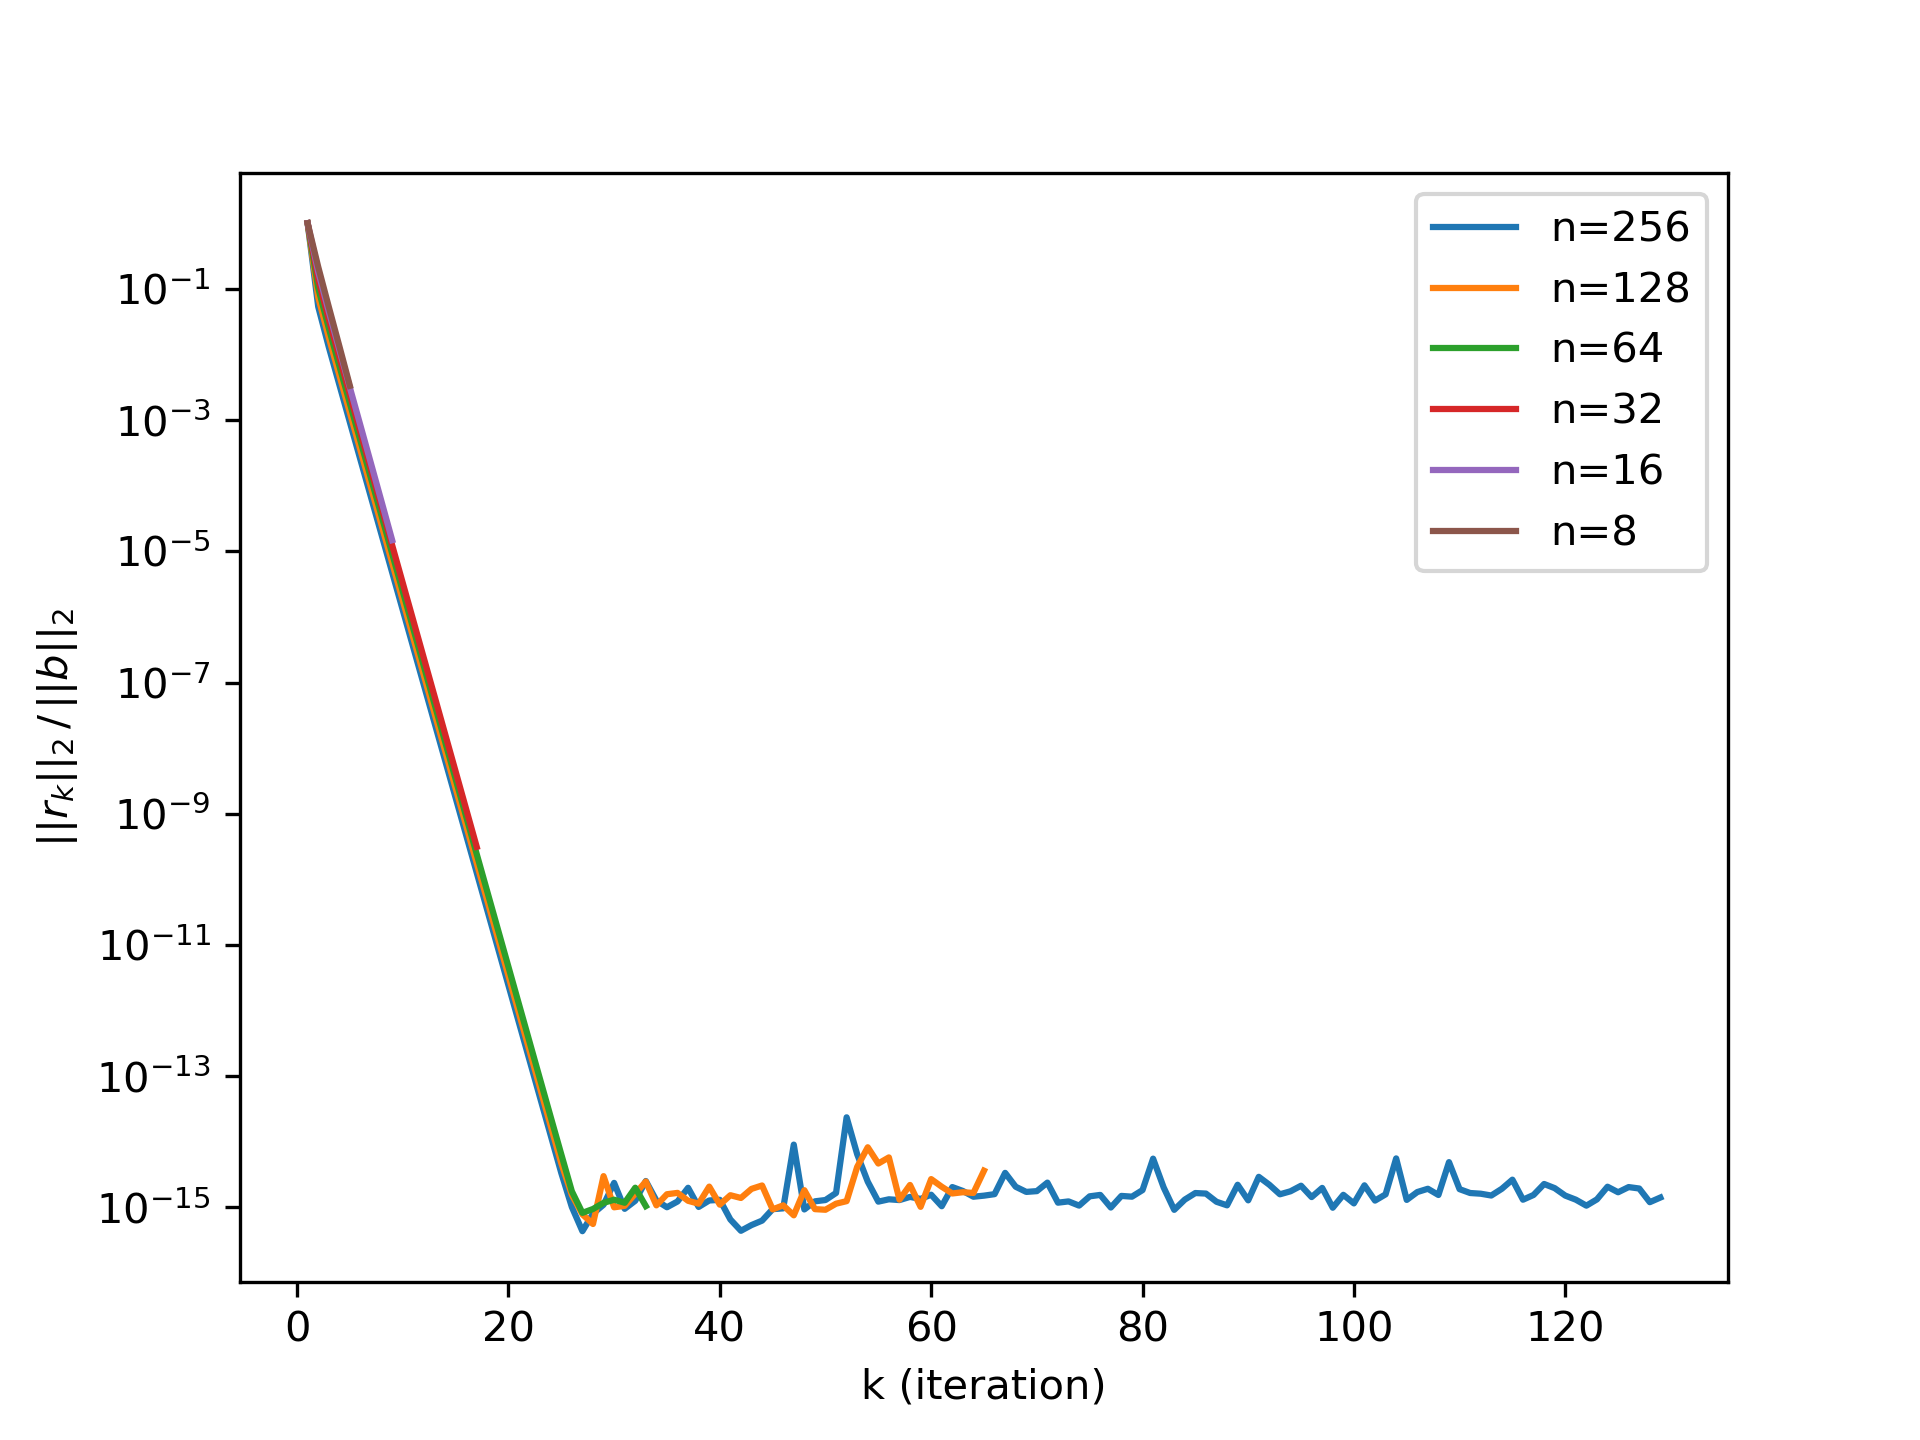
\includegraphics[width=.8\linewidth]{./q2_fig.png}
		\caption{}
    	\label{fig:q2_fig}
	\end{figure}

\section*{2.3}
		
	If I did get this part working, here is what I would have tried to do. Just looking at the
	main algorithm for gmres, without taking into account the vector and matrix operations, I dont
	think there is a way to parallelise it. The approach I would take is to write some matrix 
	multiplicationn functions, vector addition, matrix vector multiplication and parallelise them 
	with OMP since there isnt any complex message passing needed for these operations. For the 
	minimisation problem of finding y I would choose to do a qr decompostions with a gram schmidt 
	algorithm and solve the correspinding system of equations for y with that, also parallelising 
	this with OMP. Possible tests for correctednes would be comparing it with my serial implementation
	. Comparing the residuals and the actaul solution. A good stopping criteria for this algorithm
	would be to stop the algorithm once the residual is below a certain threshold, for example close to
	machine precision.

\bibliographystyle{plain} 
\bibliography{refs} 

\end{document}



